\documentclass[12pt,letterpaper,titlepage]{report}

% packages

\usepackage[utf8]{inputenc}
\usepackage{mathptmx}
\usepackage{amsmath}
\usepackage{geometry}
\usepackage{float}
\usepackage{subcaption}
\usepackage{multirow}
\usepackage{makecell}
\usepackage{circuitikz}
\usepackage{pgfplots}
\usepackage{ctable}

% commands

\newcommand{\myTitle}{Series and Parallel Circuits}
\newcommand{\myName}{Shawn Lutch}
\newcommand{\myPeriod}{PHYS 2240.502}
\pgfplotsset{compat=1.10}

% shamelessly copied and pasted from https://tex.stackexchange.com/a/229158

\ctikzset{bipoles/ammeter/text rotate/.initial=0,
rotation/.style={bipoles/ammeter/text rotate=#1}}

% code from pgfcircbipoles.sty

\makeatletter
\pgfcircdeclarebipole{}{\ctikzvalof{bipoles/ammeter/height}}{ammeter}{\ctikzvalof{bipoles/ammeter/height}}{\ctikzvalof{bipoles/ammeter/width}}{
    \def\pgf@circ@temp{right}
    \ifx\tikz@res@label@pos\pgf@circ@temp
        \pgf@circ@res@step=-1.2\pgf@circ@res@up
    \else
        \def\pgf@circ@temp{below}
        \ifx\tikz@res@label@pos\pgf@circ@temp
            \pgf@circ@res@step=-1.2\pgf@circ@res@up
        \else
            \pgf@circ@res@step=1.2\pgf@circ@res@up
        \fi
    \fi

    \pgfpathmoveto{\pgfpoint{\pgf@circ@res@left}{\pgf@circ@res@zero}}       
    \pgfpointorigin \pgf@circ@res@other =  \pgf@x  \advance \pgf@circ@res@other by -\pgf@circ@res@up
    \pgfpathlineto{\pgfpoint{\pgf@circ@res@other}{\pgf@circ@res@zero}}
    \pgfusepath{draw}

    \pgfsetlinewidth{\pgfkeysvalueof{/tikz/circuitikz/bipoles/thickness}\pgfstartlinewidth}

        \pgfscope
            \pgfpathcircle{\pgfpointorigin}{.9\pgf@circ@res@up}
            \pgfusepath{draw}       
        \endpgfscope    

    \pgftransformrotate{\ctikzvalof{bipoles/ammeter/text rotate}}% <= magic line
    \pgfsetlinewidth{\pgfstartlinewidth}

    \pgfsetarrowsend{latex}
    \pgfpathmoveto{\pgfpoint{\pgf@circ@res@other}{\pgf@circ@res@down}}
    \pgfpathlineto{\pgfpoint{-\pgf@circ@res@other}{\pgf@circ@res@up}}
    \pgfusepath{draw}
    \pgfsetarrowsend{}


    \pgfpathmoveto{\pgfpoint{-\pgf@circ@res@other}{\pgf@circ@res@zero}}
    \pgfpathlineto{\pgfpoint{\pgf@circ@res@right}{\pgf@circ@res@zero}}
    \pgfusepath{draw}


    \pgfnode{circle}{center}{\textbf{A}}{}{}
}
\makeatother % allow rotation of elements in circuit diagram

% metadata

\usepackage[pdftex,
            pdfauthor={\myName{}},
            pdftitle={\myTitle{}},
            pdfsubject={\myPeriod{}},
            pdfproducer={\myName{} via LaTeX},
            pdfcreator={pdflatex}]{hyperref}
			
% layout

\pagenumbering{gobble}
\raggedright
\geometry{
	letterpaper,
	lmargin=0.75in,
	rmargin=0.75in,
	tmargin=1.0in,
	bmargin=1.0in
}

% document

\begin{document}


%% title page


\title{\myTitle{}}
\author{\myName{}\\ \myPeriod{}}
\date{\today}
\maketitle


%% abstract


\section*{Abstract}

In this lab, we found that we were able to calculate a theoretical $R_{eq}$ to within a precision of $\pm 10\%$. We calculated $R_{eq, 1}$ within a difference of 10.48\%, $R_{eq, 2}$ within a difference of 2.55\%, $R_{eq, 3}$ within a difference of 3.81\%, and $R_{eq, 4}$ within a difference of 4.42\%.


%% introduction

\bigskip
\section*{Introduction}

\textbf{Ohm's Law (equation \ref{ohms_law})} describes the relationship between voltage, current, and resistance. Ohm's Law defines a direct proportionality between current $I$ and voltage $V$, with a constant resistance $R$.

\begin{equation} \label{ohms_law}
V = I \times R
\end{equation}

A \textbf{resistor} is a device that obeys Ohm's Law and has some resistance $R$. A complex circuit that contains multiple resistors, each with its own value for $R$, has some \textbf{equivalent resistor}. The equivalent resistor is a resistor that would produce the same total current when the same total voltage is applied. The resistance of the equivalent resistor is referred to as the \textbf{equivalent resistance} of the circuit, denoted $R_{eq}$.

\medskip
The equivalent resistor would obey Ohm's Law just as the actual resistors do. In a complex circuit that produces current $I_{total}$ when a voltage $V_{total}$ is applied, the equivalent resistance of the circuit can be calculated using a rearranged form of Ohm's Law. Using an ammeter and a fixed voltage source, we can use \textbf{equation \ref{ohms_law_rearranged}} to calculate the equivalent resistance of the circuit.

\begin{equation} \label{ohms_law_rearranged}
R_{eq} = \frac{ V_{total} }{ I_{total} }
\end{equation}

Without knowing the total voltage and total current of the circuit, we can still calculate the equivalent resistance of the circuit as long as we know the resistance of each resistor. We do this by performing calculations based on how the resistors are connected. For resistors connected in series, the resistances can simply be added together, as in \textbf{equation \ref{req_series}}. For resistors connected in parallel, we add the resistances as reciprocals, as in \textbf{equation \ref{req_parallel}}.

\begin{equation} \label{req_series}
R_{eq} = \sum_{i=1}^{n} R_{i}
\end{equation}

\begin{equation} \label{req_parallel}
\frac{1}{R_{eq}} = \sum_{i=1}^{n} \frac{1}{R_i}
\end{equation}

\bigskip
In this lab, we demonstrate the ability to calculate equivalent resistance using two methods:

\begin{enumerate}
    \item Using known values for $V_{total}$ and $I_{total}$ and equation \ref{ohms_law_rearranged}
    \item Using known values for $R_{1 \ldots n}$ and equations \ref{req_series} and \ref{req_parallel}
\end{enumerate}


%% apparatus

\pagebreak
\section*{Apparatus}

\begin{itemize}
	\item PASCO Capstone (data acquisition, display, analysis software)
	\item 850 Universal Interface
	\item AC/DC Electronics Laboratory
	\item Patch cords (x8)
	\item Resistors (x6)
		\begin{itemize}
			\item 100 $\Omega$ (brown-black-brown-gold) resistors (x2)
			\item 330 $\Omega$ (orange-orange-brown-gold) resistors (x2)
			\item 560 $\Omega$ (green-blue-brown-gold) resistors (x2)
		\end{itemize}
\end{itemize}


%% procedure

\bigskip
\section*{Experimental Procedure}

The precision of each resistor is $\pm 5 \%$, as indicated by the gold band on each. For maximum precision in our values for each circuit's $R_{eq}$, we first needed to find the actual resistance of our six resistors. These numbers would be used later in our calculations for the theoretical $R_{eq}$ of each circuit. The following circuit was used to calibrate each resistor $R_{1 \ldots 6}$ by using the PASCO Capstone software to record the actual resistance to a precision of around $\pm 1\%$.

\begin{center}
    \begin{circuitikz}
\draw
(2,2) to[battery,l=850 Interface] (2,0)
      to[ammeter,rotation=180] (0,0)
      to[resistor,l=$R_n$] (0,2) -- (2,2)
;
\end{circuitikz}
\end{center}

To account for electrical noise, which can cause error approaching 5 mA, we also calibrated the ammeter. We inserted the resistor with the closest resistance to $100 \Omega$ (which ended up being $R_4$) into the calibration circuit. Then, using the actual resistance value of $R_4$, we calculated the ideal current in a circuit powered by a range of DC voltages from 0V to 7V. We then measured and recorded the actual current of the circuit with each voltage, and notated a correction value that would be used later to account for electrical noise.

\medskip
The lab manual gave us four circuit diagrams, from which we were to build the circuits. The print was small and heavily compressed, so it was difficult to read the $R_n$ subscripts. We used the ideal resistance values given in the diagrams (not included in the reproductions on the next page) and process of elimination to figure out which resistor was supposed to be which.

\pagebreak
Below are the four circuits, as laid out in the lab manual.

\bigskip
\begin{minipage}{\textwidth}
    \centering
    \bigskip
    \begin{tabular}{| l | l |}
    \hline
    
    % circuit 1
    \begin{minipage}{.4\textwidth}
        \centering
        \bigskip
        \begin{circuitikz}
            \draw
            (0,0) to[short,o-] (0.4,0)
                  to[resistor,l=$R_2$] (2.4,0) -- (3,0)
                  to[resistor,l=$R_1$] (5,0)
                  to[short,-o] (5.4,0)
            ;
        \end{circuitikz} \\
        Circuit 1
        \bigskip
    \end{minipage} &
    
    % circuit 2
    \begin{minipage}{.4\textwidth}
        \centering
        \bigskip
        \begin{circuitikz}
            \draw
            (3,2) to[short,o-]          (2,2)
                  to[resistor,l=$R_1$]  (2,0)
                  to[short,-o]          (3,0)
            (2,2) --                    (0,2)
                  to[resistor,l=$R_2$]  (0,0)
                  --                    (2,0)
            ;
        \end{circuitikz} \\
        Circuit 2
        \bigskip
    \end{minipage} \\
    
    \hline
    
    % circuit 3
    \begin{minipage}{.4\textwidth}
        \centering
        \bigskip
        \begin{circuitikz}
            \draw
            (0,0) to[resistor,l=$R_2$] (0,2)
                  --                   (4,2)
                  to[short,-o]         (4.4,2)
            (0,0) --                   (2,0)
                  to[resistor,l=$R_1$] (2,2)
            (2,0) to[resistor,l=$R_3$] (4,0)
                  to[short,-o]         (4.4,0)
            ;
        \end{circuitikz} \\
        Circuit 3
        \bigskip
    \end{minipage} &
    
    % circuit 4
    \begin{minipage}{.4\textwidth}
        \centering
        \bigskip
        \begin{circuitikz}
            \draw
            (0,2) to[resistor,l=$R_6$] (0,0)
                  --                   (2,0)
            (0,2) to[resistor,l=$R_4$] (2,2)
                  to[resistor,l=$R_5$] (2,0)
                  --                   (4,0)
            (2,2) to[resistor,l=$R_1$] (4,2)
                  to[resistor,l=$R_2$] (4,0)
                  --                   (6,0)
                  to[short,-o]         (6.4,0)
            (4,2) to[resistor,l=$R_3$] (6,2)
                  to[short,-o]         (6.4,2)
            ;
        \end{circuitikz} \\
        Circuit 4
        \bigskip
     \end{minipage} \\
     
     \hline
        
\end{tabular}
    \bigskip
\end{minipage}

\medskip
We used equations \ref{req_series} and \ref{req_parallel} to calculate the theoretical $R_{eq}$ for each circuit. We found circuit 4 particularly troublesome, and it took some time to calculate its theoretical $R_{eq}$. Afterward, we built each of the circuits and measured the $I_{total}$ of each circuit with a constant $V_{total} =$ 15V DC. We used these values to calculate each circuit's experimental $R_{eq}$. We calculated the percent difference between theoretical and actual $R_{eq}$ values for each circuit and called it a day.

\medskip
We also discussed the difference in current and voltage between circuits in series and in parallel, as demonstrated with light bulbs. Those figures were not recorded and are not included in this lab report.



%% data

\pagebreak
\section*{Data}

% more padding, sure fuck it
\bigskip
\bigskip

% resistor calibration
\begin{minipage}{\textwidth}
    \centering
    \begin{tabular}[t]{c c}
        
        % resistor calibration
        \begin{minipage}{.4\textwidth}
            \centering
            \bigskip
            Resistance Calibration \\
            \bigskip
            \begin{tabular}{ | c | c | c | c | c | c | } \hline

    \thead{$R_n$} & \thead{Ideal \\ $R$ ($\Omega$)} & \thead{Measured \\ $R$ ($\Omega$)} \\ \hline
    $R_1$ & 330 & 315  \\ \hline
    $R_2$ & 560 & 535  \\ \hline
    $R_3$ & 100 & 95.7 \\ \hline
    $R_4$ & 100 & 96.8 \\ \hline
    $R_5$ & 560 & 537  \\ \hline
    $R_6$ & 330 & 314  \\ \hline
    
\end{tabular}
            \bigskip
            \bigskip % fuck having to have these bigskips
            \bigskip % but it's for the good of the formatting
            \bigskip
            \medskip % mix it up a bit, eh?
        \end{minipage} &
        
        % ammeter calibration
        \begin{minipage}{.4\textwidth}
            \centering
            \bigskip
            Ammeter Calibration \\
            \bigskip
            \begin{tabular}{ | c | c | c | c | } \hline
	\thead{Voltage (V)} & \thead{Theoretical \\ Current (mA)} & \thead{Measured \\ Current (mA)} & \thead{Correction \\ (mA)} \\ \hline
	0 V & 0 mA & 0.3 mA & -0.3 mA \\ \hline
	1 V & 10.3 mA & 10.6 mA & -0.3 mA \\ \hline
	2 V & 20.7 mA & 20.9 mA & 0.2 mA \\ \hline
	3 V & 31.0 mA & 31.0 mA & 0.0 mA \\ \hline
	4 V & 41.3 mA & 41.3 mA & 0.0 mA \\ \hline
	5 V & 51.7 mA & 51.6 mA & 0.1 mA \\ \hline
	6 V & 62.0 mA & 62.1 mA & -0.1 mA \\ \hline
	7 V & 72.3 mA & 72.5 mA & -0.2 mA \\ \hline
\end{tabular}
            \bigskip
            \bigskip
        \end{minipage} \\
        
        \multicolumn{2}{c} {
            \begin{minipage}{.4\textwidth}
                \centering
                \bigskip
                \bigskip
                Measured and Corrected Current \\
                \bigskip
                \begin{tabular}{ | c | c | c | c | } \hline

     \thead{Circuit} & \thead{Measured \\ Current (A)} & \thead{Corrected \\ Current (A)} \\ \hline
     
     1 & 19.8 & 19.6 \\ \hline
     2 & 77.8 & 77.6 \\ \hline
     3 & 52.9 & 53.0 \\ \hline
     4 & 42.8 & 42.8 \\ \hline
    
\end{tabular}
                \bigskip
            \end{minipage}
        }
                
    \end{tabular}
\end{minipage}

\bigskip
\bigskip


%% calcs and graphs

\pagebreak
\section*{Calculations and Graphs}

\begin{minipage}{\linewidth}
    \centering
    \bigskip    
    
    \begin{tabular}{c c}

        \begin{minipage}{.45\linewidth}
            \centering
            Calculated Resistances \\
            \bigskip
            \begin{tabular}{| c | c | c | c |} \hline
    
    \thead{Circuit} & \thead{Theor. \\ $R_{eq}$ ($\Omega$)} & \thead{Exper. \\ $R_{eq}$ ($\Omega$)} & \thead{\% \\ Diff.} \\ \hline
    
    1 & 850   & 765   & 10.48 \\ \hline
    2 & 198.3 & 193.3 & 2.55  \\ \hline
    3 & 294.0 & 283.0 & 3.81  \\ \hline
    4 & 366.4 & 350.5 & 4.42  \\ \hline
    
    
\end{tabular}
            \bigskip
            \bigskip % this
            \bigskip % stupid
            \bigskip % padding
            \bigskip % bullshit
            \bigskip % again
            \bigskip
            \medskip % lel
            \bigskip
        \end{minipage} &
        
        \begin{minipage}{.5\linewidth}
            \centering
            <<<<<<< HEAD
=======
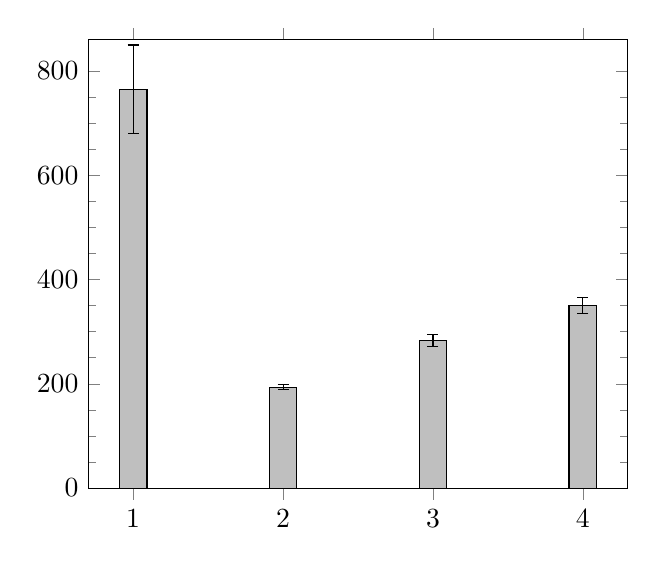
\begin{tikzpicture}

    \begin{axis}[
        xtick = { 1,...,4 },
        xticklabels = { 1, 2, 3, 4 },
        ymax = 860,
        ymin = 0,
        minor y tick num = 3,
        ybar
    ]
    
        \addplot[
            fill = black!25,
            draw = black,
            error bars/.cd,
            y dir = both,
            y explicit
        ]
        table [y error = error] {
            x  y      error  label
            1  765.3  84.7   1
            2  193.3  5.0    2
            3  283.0  11.0   3
            4  350.5  15.9   4
        };
        
    \end{axis}

\end{tikzpicture}
>>>>>>> parent of 88fa715... replace error bars in resistance histogram with second set of data

        \end{minipage}

    \end{tabular}    
\end{minipage}

\bigskip
\bigskip


%% discussion

\bigskip
\section*{Discussion of Results and Error Analysis}

% how well did the theoretical values compare to the experimental values?

In general, our calculated theoretical values were close to the measured experimental values within a reasonable margin of error. We found that we were able to calculate the theoretical $R_{eq}$ with around $\pm 5\%$ difference from the experimental $R_{eq}$, with the exception of Circuit 1, which had a 10.48\% difference between the two.

\medskip

% what are sources of error in this experiment, and how could they be minimized?

Currently, it is not clear why our theoretical $R_{eq}$ varies so wildly from the experimental $R_{eq}$ in Circuit 1, although the main source of error throughout the entire experiment was electrical noise from the voltage source. Although we corrected for discrepancies in current, electrical noise is not uniform, and is difficult to predict and correct for.


%% conclusion

\bigskip
\section*{Conclusion}


%% done...


\end{document}